%!TEX program = xelatex

\documentclass[compress]{beamer}
%--------------------------------------------------------------------------
% Common packages
%--------------------------------------------------------------------------
\usepackage[english]{babel}
\usepackage{pgfpages} % required for notes on second screen
\usepackage{graphicx}
\usepackage{subfigure}
\usepackage{multicol}
\usepackage{multirow}
\def\block(#1,#2)#3{\multicolumn{#2}{c}{\multirow{#1}{*}{$ #3 $}}}

\usepackage{fontspec}

\usepackage{tabularx,ragged2e}
\usepackage{booktabs}

\usepackage{setspace}

%--------------------------------------------------------------------------
% Load theme
%--------------------------------------------------------------------------
\usetheme{hri}

\usepackage{dtklogos} % must be loaded after theme
\usepackage{tikz}
\usetikzlibrary{intersections,arrows,shapes,calc,mindmap,backgrounds,positioning,svg.path}

\graphicspath{{figs/}}


\usepackage[cache]{minted}
\renewcommand{\theFancyVerbLine}{
  \sffamily\textcolor[rgb]{0.5,0.5,0.5}{\scriptsize\arabic{FancyVerbLine}}}

\newminted{glsl}{linenos=false,
                 fontsize=\tiny}

\newcount\colveccount
\newcommand*\colvec[1]{
        \global\colveccount#1
        \begin{bmatrix}
        \colvecnext
}
\def\colvecnext#1{
        #1
        \global\advance\colveccount-1
        \ifnum\colveccount>0
                \\
                \expandafter\colvecnext
        \else
                \end{bmatrix}
        \fi
}

\tikzset{box/.style={
            draw, 
            fill=blue!20,
            fill opacity=0.8,
            thick,
            inner sep=0pt,
            minimum size=1cm,
            transform shape
        },
        finalbox/.style={
            draw, 
            fill=orange,
            fill opacity=0.8,
            thick,
            inner sep=0pt,
            minimum size=1cm,
            transform shape
        },
        dot/.style={
            draw,
            circle,
            fill=red!20,
            inner sep=0pt,
            minimum size=1cm,
            transform shape
        },
        axis/.style={
            thick,
            gray,
            font=\small},
        every to/.style={
            >=latex,
            dashed,
            thick
        }
    }



%--------------------------------------------------------------------------
% General presentation settings
%--------------------------------------------------------------------------
\title{Introduction à l'infographie 3D}
\subtitle{CS211 -- Introduction à l'informatique visuelle}
\date{24 février 2015}
\author{Séverin Lemaignan}
\institute{Computer-Human Interaction\\for Learning and Instruction {\Medium
EPFL}}

%--------------------------------------------------------------------------
% Notes settings
%--------------------------------------------------------------------------
%\setbeameroption{show notes on second screen}
%\setbeameroption{hide notes}

\begin{document}

\maketitle

%%%%%%%%%%%%%%%%%%%%%%%%%%%%%%%%%%%%%%%%%%%%%%%%%%%%%%%%%%%%%%%%%%%%%%%%%%%%%%%
\begin{frame}{Au commencement, le point...}
    \begin{center}
    \only<1>{
        \input{sketches/point.tex}
    }
    \only<2>{
        \input{sketches/points.tex}
    }
    \only<3>{
        \input{sketches/cube.tex}
    }

    \only<4>{
        \input{sketches/scene-graph-only-cube.tex}
    }

    \only<5>{
        \input{sketches/world.tex}
    }
    \end{center}


\end{frame}

\imageframe{dieu.png}

\begin{frame}{}
    \begin{center}
        Et Dieu nomma le point...\\[1em]
        \uncover<2>{
        \Large
    $\begin{bmatrix} x \\ y \\ z \end{bmatrix}$

        \scriptsize
        (et il nota au passage que le point appartenait à $\mathbb{R}^3$)
    }
    \end{center}

\end{frame}

\begin{frame}{}
    \begin{center}
        Et il vit que c'était très réussi.\\[1em]

        Alors il nomma le monde...\\[1em]

        \uncover<2>{
        \Large
        Base canonique $\{\vec{e_1}, \vec{e_2}, \ldots, \vec{e_n}\}$,
    }
    \end{center}

\end{frame}

\begin{frame}{}
    \begin{center}
        (c'était moins réussi)\\[1em]

        Alors il se dit que, en 3D,...\\[1em]

        \uncover<2>{
        \Large
    $\{\vec{u}, \vec{v}, \vec{w} \} = \left \{\begin{bmatrix} 1 \\ 0 \\ 0 \end{bmatrix},
    \begin{bmatrix} 0 \\ 1 \\ 0 \end{bmatrix},
    \begin{bmatrix} 0 \\ 0 \\ 1 \end{bmatrix}\right \}$
        \\[1em]
        \normalsize
        ça irait bien aussi.
    }
    \end{center}

\end{frame}

\begin{frame}{}
    Ensuite, Dieu se gratta le menton : \\[1em] 
    Comment placer tous ces points dans le monde ? \\[2em]

    \uncover<2>{
        Alors il créa Sintel...
    }
\end{frame}

\imageframe{sintel-vertices.png}
\imageframe{sintel-wireframe.png}
\imageframe{sintel-opengl.png}
\imageframe{sintel-opengl-textures.png}
\imageframe{sintel.png}

\begin{frame}{}
    \begin{center}
        ({\Medium Sintel}, c'est un court métrage d'animation 3D, réalisé avec Blender, et
    complètement open-source.\\
    
    Vous pouvez télécharger tout le {\Medium source} du
    film (modèles 3D, textures,...) sur
    \url{https://durian.blender.org/})
    \end{center}
\end{frame}

\begin{frame}{}
    \begin{center}
Plus sérieusement :
    \end{center}
        \tableofcontents
\end{frame}
%%%%%%%%%%%%%%%%%%%%%%%%%%%%%%%%%%%%%%%%%%%%%%%%%%%%%%%%%%%%%%%%%%%%%%%%%%%%%%%

\section[Transformations]{Transformations linéaires}

\begin{frame}{}
    \begin{center}
\Large
\[
    T(\mathbf{x}) = A \cdot \mathbf{x}
\]
\[
    T(\mathbf{x}) = A \cdot \mathbf{x} + B
\]
\normalsize
\uncover<2->{
    \\[2em]
    $\mathbf{x}$ dénote une variable quelconque. Par exemple, le vecteur $\vec
    a = [a_0, a_1, \ldots, a_n]$. Ou bien le vecteur $\vec x = [x,y,z]$.
}
\uncover<3>{
    \\[2em]
    Si $\mathbf{x}$ et $T(\mathbf{x})$ sont des vecteurs, alors $A$ (et $B$)
    sont probablement des matrices !
}
    \end{center}

\end{frame}

\begin{frame}{}

Pour commencer, on se place dans le plan ($\mathbb{R}^2$):

\[
\mathbf{x} = \vec{x} = \begin{bmatrix} x \\ y \end{bmatrix}
\]

\end{frame}

\begin{frame}{Expression matricielle des homothéties}

\begin{center}
\[
\vec{x'} = T( \vec{x} ) =  2 \vec{x} 
\]
\uncover<2->{
\[
\begin{bmatrix} x' \\ y' \end{bmatrix} =
    T( \vec{x} ) =\mathbf{A} \vec x = 2 \mathbf{I} \vec{x} = \begin{bmatrix} 2 && 0 \\ 
                                             0 && 2
\end{bmatrix} \begin{bmatrix} x \\ y \end{bmatrix}
\]

}

\begin{tikzpicture}
    \draw[axis,->] (0,0) -- (1.5,0) node[right] {x};
    \draw[axis,->] (0,0) -- (0,1.5) node[right] {y};

    \draw[axis,->] (4,0) -- (5.5,0) node[right] {x};
    \draw[axis,->] (4,0) -- (4,1.5) node[right] {y};

    \draw[dashed, thick, ->] (1.7,0.5) -- (3.4,0.5);

    \only<3->{
        \node[box] at (0.5,0.5) (base) {};
        \node[finalbox,cm={2,0,0,2,(0,0)}] at (5,1) (transformed) {};

        \draw (0,1) node[inner sep=0,minimum size=0.3cm,draw,circle,fill=yellow] {};
        \draw (1,0) node[inner sep=0,minimum size=0.3cm,draw,circle,fill=yellow] {};

        \draw (4,2) node[inner sep=0,minimum size=0.3cm,draw,circle,fill=red] {};
        \draw (6,0) node[inner sep=0,minimum size=0.3cm,draw,circle,fill=red] {};
    }

    \draw (1,1) node[inner sep=0,minimum size=0.3cm,draw,circle,fill=yellow] {};
    \draw (6,2) node[inner sep=0,minimum size=0.3cm,draw,circle,fill=red] {};

    \only<1-2>{
        \draw[thick,->] (0,0) -- (1,1) node[midway,left] {$\vec{x}$};
        \draw[thick,->] (4,0) -- (6,2) node[midway,left] {$\vec{x'}$};
    }


\end{tikzpicture}

\end{center}
\end{frame}

\begin{frame}{Matrices de rotation}

\[
    \left\{
        \begin{array}{lr}
            x' = x \cos \theta + y \sin\theta \\
            y' =  -x \sin \theta + y \cos\theta
        \end{array}
    \right.
\]

    \uncover<2->{
\[
    \begin{bmatrix} x' \\ y' \end{bmatrix} = \begin{bmatrix} \cos \theta &
    -\sin\theta \\ \sin \theta & \cos \theta \end{bmatrix} \begin{bmatrix} x \\ y
    \end{bmatrix}
\]
}
\uncover<1->{
    \centering
    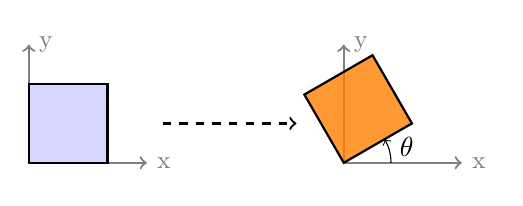
\begin{tikzpicture}
        \draw[axis,->] (0,0) -- (1.5,0) node[right] {x};
        \draw[axis,->] (0,0) -- (0,1.5) node[right] {y};

        \draw[axis,->] (4,0) -- (5.5,0) node[right] {x};
        \draw[axis,->] (4,0) -- (4,1.5) node[right] {y};

        \draw[dashed, thick, ->] (1.7,0.5) -- (3.4,0.5);

        \node[box] at (0.5,0.5) (base) {};
        \node[finalbox,rotate around={30:(-0.5,-0.5)}] at (4.5,0.5) (transformed) {};

        \draw[solid,->] (4.6,0) arc(0:30:0.6);
        \node at (4.8,0.2) {$\theta$};

    \end{tikzpicture}

}
\end{frame}

\begin{frame}{Cisaillement (shearing)}
    \begin{multicols}{2}

\[
\begin{bmatrix} x' \\ y' \end{bmatrix} = \begin{bmatrix} 1 & k \\ 0 & 1
\end{bmatrix} \begin{bmatrix} x \\ y \end{bmatrix}
\]
    \centering
    
\begin{tikzpicture}
       \node[box] at (0,0) (base) {};
        \node[finalbox,cm={1,0,1,1,(0,0)}] at (3,0) (transformed) {};
        \draw[dashed, thick, ->] (1,0) -- (2,0);
    \end{tikzpicture}

    \end{multicols}

    \begin{multicols}{2}

\[
\begin{bmatrix} x' \\ y' \end{bmatrix} = \begin{bmatrix} 1 & 0 \\ k & 1
\end{bmatrix} \begin{bmatrix} x \\ y \end{bmatrix}
\]
    \centering
    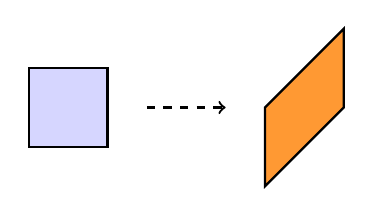
\begin{tikzpicture}
        \node[box] at (0,0) {};
        \node[finalbox,cm={1,1,0,1,(0,0)}] at (3,0) {};
        \draw[dashed, thick, ->] (1,0) -- (2,0);
    \end{tikzpicture}

    \end{multicols}


\end{frame}

\begin{frame}{}

Quelle transformation représente la matrice ci-dessous ?

\[
\begin{bmatrix} x' \\ y' \end{bmatrix} = \begin{bmatrix} 1 & 0 \\ 0 & 0
\end{bmatrix} \begin{bmatrix} x \\ y \end{bmatrix}
\uncover<2>{
= \begin{bmatrix} x \\ 0 \end{bmatrix} 
}
\]

\end{frame}

\begin{frame}{}
    Dans $\mathbb{R}^3$,
\[
    T( \vec{x} ) = \begin{bmatrix} 2 & 0 & 0 \\ 
                                   0 & 2 & 0 \\
                                   0 & 0 & 2 
\end{bmatrix} \vec{x} 
= \begin{bmatrix} 2 & 0 & 0 \\ 
                                   0 & 2 & 0 \\
                                   0 & 0 & 2 
\end{bmatrix} 
\begin{bmatrix} x \\ y \\ z \end{bmatrix}
\]

\uncover<2->{
De manière générale, comment construire $\mathbf{A}$ qui représente la
transformation linéaire $T(\mathbf{x})$ ?
}
\uncover<3->{

\begin{align*}
\mathbf{A} &= \begin{bmatrix} T( \vec u ) & T( \vec v ) & T( \vec w ) \end{bmatrix}
\\
&= \begin{bmatrix}
T\left (\begin{bmatrix} 1 \\ 0 \\ 0 \end{bmatrix}\right ) &
T\left (\begin{bmatrix} 0 \\ 1 \\ 0 \end{bmatrix}\right ) &
T\left (\begin{bmatrix} 0 \\ 0 \\ 1 \end{bmatrix} \right ) \end{bmatrix}
\end{align*}
}
\end{frame}

\begin{frame}{}

    Représenter les transformations sous forme matricielle est particulièrement
    efficace (opérations ne requiérant que des multiplications et des additions,
    vectorisation via SSE).

    \uncover<2->{
    \LARGE
    Mais pour les transformations {\Medium non linéaires}? \\[1em]
    \normalsize
    Par ex., les
    {\Medium transformations affines} $T(\mathbf{x}) = A \cdot \mathbf{x} + B$, comme les
    translations.
    }

\end{frame}


%%%%%%%%%%%%%%%%%%%%%%%%%%%%%%%%%%%%%%%%%%%%%%%%%%%%%%%%%%%%%%%%%%%%%%%%%%%%%%%

\section{Coordonnées homogènes}



\begin{frame}{Intuition}
    \only<1-4>{
    \[
    \begin{bmatrix} x' \\ y' \end{bmatrix} = \begin{bmatrix} 1 & k \\ 0 & 1
    \end{bmatrix} \begin{bmatrix} x \\ y \end{bmatrix}
    \]
    }
    \only<1>{
    \centering
    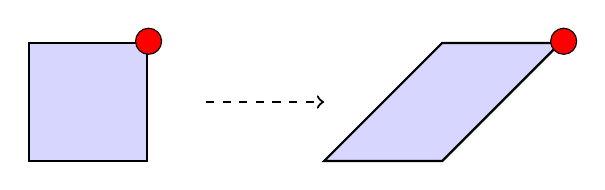
\begin{tikzpicture}[scale=1.5]
        \node[box] at (0,0) (base) {};
        \node[box,cm={1,0,1,1,(0,0)}] at (3,0) (transformed) {};
        \draw (base.north east) node[minimum size=0.1cm,draw,circle,fill=red] {};
        \draw (transformed.north east) node[minimum size=0.1cm,draw,circle,fill=red] {};
        \draw[dashed, thick, ->] (1,0) -- (2,0);
    \end{tikzpicture}

    }
    \only<2>{
        \centering
    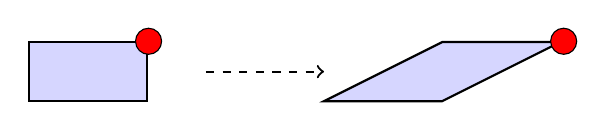
\begin{tikzpicture}[scale=1.5]
        \begin{scope}[cm={1,0,0,0.5,(0,0)}]
            \node[box] at (0,0) (base) {};
            \node[box,cm={1,0,1,1,(0,0)}] at (3,0) (transformed) {};
        \end{scope}
        \draw (base.north east) node[minimum size=0.1cm,draw,circle,fill=red] {};
        \draw (transformed.north east) node[minimum size=0.1cm,draw,circle,fill=red] {};
        \draw[dashed, thick, ->] (1,0) -- (2,0);
    \end{tikzpicture}
    }
    \only<3>{
        \centering

    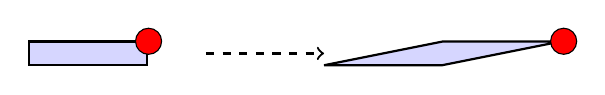
\begin{tikzpicture}[scale=1.5]
        \begin{scope}[cm={1,0,0,0.2,(0,0)}]
            \node[box] at (0,0) (base) {};
            \node[box,cm={1,0,1,1,(0,0)}] at (3,0) (transformed) {};
        \end{scope}
        \draw (base.north east) node[minimum size=0.1cm,draw,circle,fill=red] {};
        \draw (transformed.north east) node[minimum size=0.1cm,draw,circle,fill=red] {};
        \draw[dashed, thick, ->] (1,0) -- (2,0);
    \end{tikzpicture}
    
    }
    \only<4>{
        \centering

    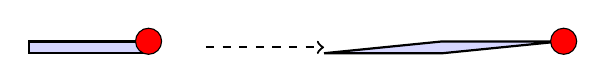
\begin{tikzpicture}[scale=1.5]
        \begin{scope}[cm={1,0,0,0.1,(0,0)}]
            \node[box] at (0,0) (base) {};
            \node[box,cm={1,0,1,1,(0,0)}] at (3,0) (transformed) {};
        \end{scope}
        \draw (base.north east) node[minimum size=0.1cm,draw,circle,fill=red] {};
        \draw (transformed.north east) node[minimum size=0.1cm,draw,circle,fill=red] {};
        \draw[dashed, thick, ->] (1,0) -- (2,0);
    \end{tikzpicture}

    }
    \only<5>{
        \centering
        \video{0.7\textwidth}{videos/affine_transformations.ogv}\\
        \vspace*{1em}
    }

    \uncover<6->{
        {\Medium Idée clé} : ajouter une dimension (\emph{coordonnée $w$}) pour linéariser les {\Medium transformations
        affines} (comme les translations) et les {\Medium transformations
        projectives} (on va y revenir).
    }
\end{frame}

\begin{frame}{}
\[
\begin{bmatrix} x' \\ y' \\ 1 \end{bmatrix} = \begin{bmatrix} 1 & 0 & t_x \\ 0
                                                                 & 1 & t_y \\ 0
                                                                 & 0 & 1
\end{bmatrix} \begin{bmatrix} x \\ y \\ 1 \end{bmatrix} = \begin{bmatrix} x +
    t_x \\ y + t_y
\\ 1 \end{bmatrix}
\]

\uncover<2-> {
    Une translation en 2D (transformation affine) peut être représentée comme un
    cisaillement en 3D (transformation linéaire).
}
\end{frame}

\begin{frame}{Espace projectif et coordonnées homogènes}


$\begin{bmatrix} x \\ y \\ 1 \end{bmatrix}$ représente {\Medium une} des
{\Medium coordonnées homogènes} du point $\begin{bmatrix} x \\ y \end{bmatrix}$
dans {\Medium l'espace projectif} associé à l'espace euclidien
$\mathbb{R}^2$.\\[1em]

\uncover<2->{
$\begin{bmatrix} k\ x \\ k\ y \\ k \end{bmatrix}, k \in \mathbb{R}\setminus\{0\}$ représente {\Medium l'ensemble des coordonnées homogènes} du point
$(x, y)$.\\[1em]
}

\uncover<3->{
Pour repasser en coordonnées euclidiennes, il suffit de diviser par la
coordonnée $w$ ({\Medium normalisation}) : $\begin{bmatrix} x \\ y \\ w \end{bmatrix} \cong \begin{bmatrix} x/w \\ y/w \\ 1 \end{bmatrix}$.
}

\end{frame}

\begin{frame}{Espace projectif et coordonnées homogènes}
    Exemples:

\[
\begin{bmatrix} 9 \\ 12 \\ 3 \end{bmatrix} \cong \begin{bmatrix} 45 \\ 60 \\ 25
\end{bmatrix} \cong \begin{bmatrix} 3 \\ 4 \\ 1 \end{bmatrix}
\]

\[
\begin{bmatrix} 0 \\ -2 \\ -3 \end{bmatrix} \cong \begin{bmatrix} 0 \\ 0.66... \\ 1 \end{bmatrix}
\]


\end{frame}
\begin{frame}{Coordonnées homogènes (2)}
    \centering
    Si $\begin{bmatrix} x \\ y \\ 1 \end{bmatrix}$ est un point 2D, que penser
    de $\begin{bmatrix} x \\ y \\ 0 \end{bmatrix}$?

        \uncover<2->{
        \Large
            Point à l'infini\\
            ou direction\\
            ou vecteur
        }

            \uncover<3->{
                \normalsize
        L'espace projectif permet \emph{d'équiper l'espace euclidien
        avec des points à l'infini}
    }

\end{frame}

\begin{frame}{En 3D}


\only<1>{

Coordonnées homogènes: $[x, y, z, w]^\intercal$

Translations :
\[
\begin{bmatrix} x' \\ y' \\ z' \\ 1 \end{bmatrix} = \begin{bmatrix} 1 & 0 & 0 & t_x \\
                                                                    0 & 1 & 0 & t_y \\
                                                                    0 & 0 & 1 & t_z \\
                                                                    0 & 0 & 0 & 1
\end{bmatrix} \begin{bmatrix} x \\ y \\ z \\ 1 \end{bmatrix} = \begin{bmatrix} x +
    t_x \\ y + t_y \\ z + t_z \\ 1 \end{bmatrix}
\]

Rotations :

\[
\begin{bmatrix} x' \\ y' \\ z' \\ 1 \end{bmatrix} = \begin{bmatrix}
    \block(3,3){R_{3 \times 3}} & 0 \\
                 &  &  & 0 \\
                 &  &  & 0 \\
                 0 & 0  & 0 & 1
\end{bmatrix} \begin{bmatrix} x \\ y \\ z \\ 1 \end{bmatrix}
\]
}

\only<2>{
    Homothétie (isotropique si $\alpha = \beta = \gamma$, anisotropique sinon):
\[
\begin{bmatrix} x' \\ y' \\ z' \\ 1 \end{bmatrix} = \begin{bmatrix} \alpha & 0 & 0 & 0 \\
                                                                    0 & \beta & 0 & 0 \\
                                                                    0 & 0 & \gamma & 0 \\
                                                                    0 & 0 & 0 & 1
\end{bmatrix} \begin{bmatrix} x \\ y \\ z \\ 1 \end{bmatrix} = \begin{bmatrix} \alpha x \\ \beta y \\ \gamma z \\ 1 \end{bmatrix}
\]


}

\end{frame}

\section[Composition]{Composition de transformations}

\begin{frame}{Composition de transformations}
    Simple multiplication de matrices !
    $\mathbf{B}(\mathbf{A} \vec{x} ) = (\mathbf{BA}) \vec{x}$

    \uncover<2->{
        Attention : la multiplication de matrices est associative, mais
        {\Medium pas commutative} en général!
        

        Rotation $\mathbf{A}$ suivie de Translation $\mathbf{B}$ $\equiv \mathbf{BA}\vec{x}$ et non
        $\mathbf{AB}\vec{x}$!

    \begin{multicols}{2}
    \centering
    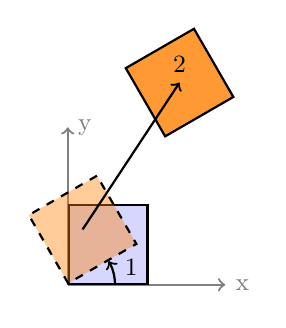
\begin{tikzpicture}[every node/.style={anchor=south west}]
        \draw[axis,->] (0,0) -- (2,0) node[right] {x};
        \draw[axis,->] (0,0) -- (0,2) node[right] {y};

        \node[box] at (0,0) (base) {};
        \begin{scope}[rotate=30]
            \node[box,dashed, fill opacity=0.4, fill=orange] at (0,0) (mid) {};
            \node[finalbox, cm={1,0,0,1,(2,1)}] at (0,0) (final) {};
        \end{scope}
        \draw[thick,->] (0.6,0) arc(0:30:0.6);
        \node at (.6,0) {\small 1};
        \draw[thick, ->] (mid.center) -- (final.center) node[above] {\small 2};


    \end{tikzpicture}
\vfill
\columnbreak
\vspace*{\fill}
    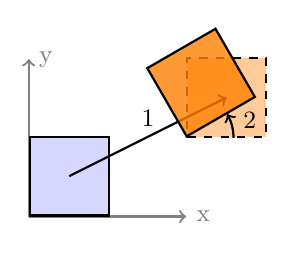
\begin{tikzpicture}[every node/.style={anchor=south west}]
        \draw[axis,->] (0,0) -- (2,0) node[right] {x};
        \draw[axis,->] (0,0) -- (0,2) node[right] {y};

        \node[box] at (0,0) (base) {};
        \begin{scope}[cm={1,0,0,1,(2,1)}]
            \node[box,dashed, fill opacity=0.4, fill=orange] at (0,0) (mid) {};
            \draw[thick, ->] (base.center) -- (mid.center) node[midway,above] {\small 1};
            \node[finalbox, rotate=30] at (0,0) (final) {};
        \end{scope}

        \draw[thick,->] (2.6,1) arc(0:30:0.6);
        \node at (2.6,1) {\small 2};

    \end{tikzpicture}


    \end{multicols}


    }
\end{frame}

\begin{frame}{Matrices de transformation généralisées}

\[
\begin{bmatrix} 1 & 0 & t_x \\
                0 & 1 & t_y \\
                0 & 0 & 1
\end{bmatrix} 
\begin{bmatrix} 
            \cos \theta  & \sin\theta & 0 \\ 
           -\sin \theta & \cos \theta & 0 \\
            0 & 0 & 1
\end{bmatrix}
\only<1>{
= ?
}
\uncover<2->{
= \begin{bmatrix} 
            \cos \theta  & \sin\theta & t_x \\ 
           -\sin \theta & \cos \theta & t_y \\
            0 & 0 & 1
\end{bmatrix}
}
\]

\uncover<3->{

\[
\begin{bmatrix} \alpha & 0 & 0 \\
                0 & \beta & 0 \\
                0 & 0 & 1
\end{bmatrix} 
\begin{bmatrix} 1 & 0 & t_x \\
                0 & 1 & t_y \\
                0 & 0 & 1
\end{bmatrix} 
\begin{bmatrix} 
            \cos \theta  & \sin\theta & 0 \\ 
           -\sin \theta & \cos \theta & 0 \\
            0 & 0 & 1
\end{bmatrix}
= \begin{bmatrix} 
            \alpha \cos \theta  & \sin\theta & t_x \\ 
           -\sin \theta & \beta \cos \theta & t_y \\
            0 & 0 & 1
\end{bmatrix}
\]

\uncover<4->{
    \centering
    \Large
    {\Medium Dans quel ordre ?}
}
}

   %\input{sketches/transformations-base.tex}

\end{frame}

\begin{frame}{Matrices de transformations généralisées en 3D}
\begin{center}
\[
\begin{bmatrix} x' \\ y' \\ z' \\ 1 \end{bmatrix} = \begin{bmatrix}
    \block(3,3){R_{3 \times 3}} & \block(1,3){T_{1 \times 3}} \\
                 &  &  &  \\
                 &  &  &  \\
                 0 & 0  & 0 & 1
\end{bmatrix} \begin{bmatrix} x \\ y \\ z \\ 1 \end{bmatrix}
\]

\uncover<2->{
\Large
Représentation standard des transformations dans l'espace (OpenGL, Direct3D...)
}
\end{center}
\end{frame}


\begin{frame}{Note : Rotations en 3D}

\only<1>{
    Les rotations dans l'espace sont difficiles à représenter !
}

\only<2>{
    Dans l'espace, une rotation $\theta$ autour de l'axe défini par le vecteur
    $\vec e = (e_x, e_y, e_z)$:

    \begin{center}
        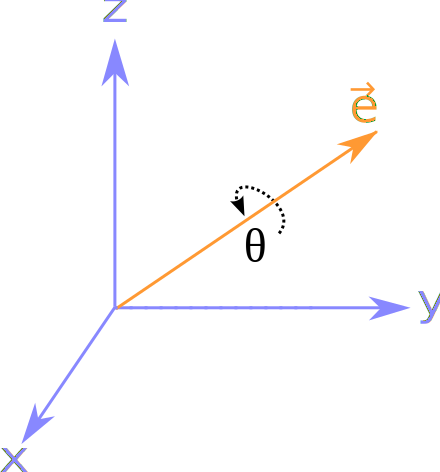
\includegraphics[width=0.4\linewidth]{rotation3d}
    \end{center}
    \[
        \left[\begin{smallmatrix}
            e_xe_x(1-\cos \theta)+\cos\theta & e_ye_x(1-\cos\theta)-e_z\sin\theta &
            e_ze_x(1-\cos\theta)+e_y\sin\theta\\
            e_xe_y(1-\cos\theta)+e_z\sin\theta & e_ye_y(1-\cos\theta)+\cos\theta &
            e_ze_y(1-\cos\theta)-e_x\sin\theta \\
            e_xe_z(1-\cos\theta)-e_y\sin\theta & e_ye_z(1-\cos\theta)+e_x\sin\theta &
            e_ze_z(1-\cos\theta)+\cos\theta
    \end{smallmatrix}\right]
    \]
}

\only<3>{
\begin{align*}
R_x(\theta) &= \begin{bmatrix}
1 & 0 & 0 \\
0 & \cos \theta &  -\sin \theta \\[3pt]
0 & \sin \theta  &  \cos \theta \\[3pt]
\end{bmatrix} \\[6pt]
R_y(\theta) &= \begin{bmatrix}
\cos \theta & 0 & \sin \theta \\[3pt]
0 & 1 & 0 \\[3pt]
-\sin \theta & 0 & \cos \theta \\
\end{bmatrix} \\[6pt]
R_z(\theta) &= \begin{bmatrix}
\cos \theta &  -\sin \theta & 0 \\[3pt]
\sin \theta & \cos \theta & 0\\[3pt]
0 & 0 & 1\\
\end{bmatrix}
\end{align*}

\[
    \mathbf{R} = \mathbf{R}_z(\theta_z) \, \mathbf{R}_y(\theta_y) \,
    \mathbf{R}_x(\theta_x) ?
\]
}

\only<4>{
    \begin{center}
        Angles d'Euler ($\varphi,\theta,\psi$) : $\mathbf{R} =
        \mathbf{R}_{z''}(\psi) \, \mathbf{R}_{x'}(\theta) \, \mathbf{R}_z(\varphi)$

        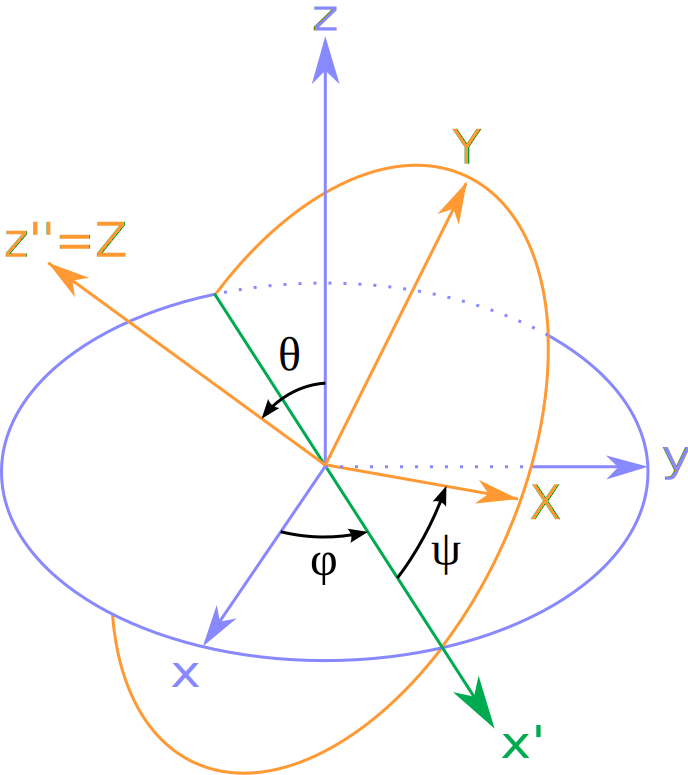
\includegraphics[width=0.5\textwidth]{eulerangles.pdf}
    \end{center}
}
\only<5>{

    Quaternions (étroitement liés aux nombres complexes) :

\[
\mathbf{q} = \begin{bmatrix}q_x \\ q_y \\ q_z \\ w \end{bmatrix}
\]
\begin{align*}
     q_x &= e_x\sin\left(\frac{\theta}{2}\right)\\
     q_y &= e_y\sin\left(\frac{\theta}{2}\right)\\
     q_z &= e_z\sin\left(\frac{\theta}{2}\right)\\
     w &= \cos\left(\frac{\theta}{2}\right)
\end{align*}

}

\end{frame}

\begin{frame}{Rotations 3D: en résumé}
    \begin{itemize}
        \item {\Medium Quaternions} : très bonnes propriétés mathématiques, peu
            intuitifs
        \item {\Medium Matrices de rotation} : bonnes propriétés mathématiques, courantes,
            peu intuitives
        \item {\Medium Angles d'Euler} : (parfois) intuitifs, mathématiquement dangeureux
        \item Autres formalismes, souvent domaine-spécifique
            (\emph{yaw-pitch-roll})
    \end{itemize}

    {\Medium Questions à l'examen : uniquement sur le vocabulaire}
\end{frame}

\begin{frame}{Scene Graph}
    \begin{center}
    \only<1>{
    \input{sketches/scene-graph-only-cube.tex}
}
     \only<2>{
    \input{sketches/scene-graph-cube.tex}
}
    \only<3->{
    \input{sketches/scene-graph.tex}
}

    \uncover<4->{
        \texttt{pushMatrix()}, \texttt{popMatrix()}!
    }
    \end{center}
\end{frame}
%%%%%%%%%%%%%%%%%%%%%%%%%%%%%%%%%%%%%%%%%%%%%%%%%%%%%%%%%%%%%%%%%%%%%%%%%%%%%%%

\section[Projections]{Les projections}


\begin{frame}{Projection}
    \begin{center}
        \includegraphics[width=0.8\linewidth]{durer-projection}
    \end{center}
\end{frame}

\begin{frame}{}
    Projection $\equiv$ fonction idempotente $\equiv P \cdot P = P$
\end{frame}

\begin{frame}{Rappel: Produit scalaire}
    \begin{center}

\[
    \vec{a} \cdot \vec{b} = \colvec{3}{a_x}{a_y}{a_z} \cdot
    \colvec{3}{b_x}{b_y}{b_z} = \| \vec{a} \| \| \vec{b} \| cos \theta = a_x b_x + a_y b_y + a_z b_z 
\]

    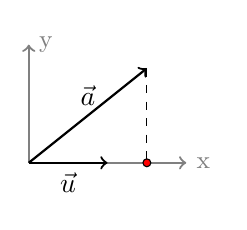
\begin{tikzpicture}
        \draw[axis,->] (0,0) -- (2,0) node[right] {x};
        \draw[axis,->] (0,0) -- (0,1.5) node[right] {y};

        \draw[thick,->] (0,0) -- (1.5,1.2) node[above,midway]{$\vec{a}$};
        \draw[thick,->] (0,0) -- (1,0) node[below,midway]{$\vec{u}$};
        \draw[thin, dashed] (1.5,1.2) -- (1.5,0) {};

        \draw (1.5,0) node[inner sep=0,minimum size=0.1cm,draw,circle,fill=red] {};

    \end{tikzpicture}

    Projection de $\vec{a}$ sur $\vec{u}$ : $(\vec a \cdot \vec u) \vec u$

    \uncover<2>{
        Que se passe-t'il pour des vecteurs orthogonaux ?
    }
    \end{center}
\end{frame}

\begin{frame}{Projection orthographique}
    \begin{center}

\[
\begin{bmatrix} 1 & 0 & 0 \\ 
                0 & 1 & 0 \\
                0 & 0 & 0
\end{bmatrix} \begin{bmatrix} x \\ y \\ z \end{bmatrix}
= \begin{bmatrix} x \\ y \\ 0 \end{bmatrix} 
\]

\only<2>{
    \input{sketches/orthoprojection.tex}
}

\only<3->{
    \input{sketches/isoprojection.tex}
}
\uncover<4->{
    Transformation linéaire
}

\end{center}
\end{frame}

\begin{frame}{Projection perspective}
    \begin{center}
    \input{sketches/projection.tex}

    \end{center}
\end{frame}

\begin{frame}{Projection perspective}
    \begin{center}
    \input{sketches/projection-cube.tex}

    \end{center}
\end{frame}



\begin{frame}{}

    \begin{center}

    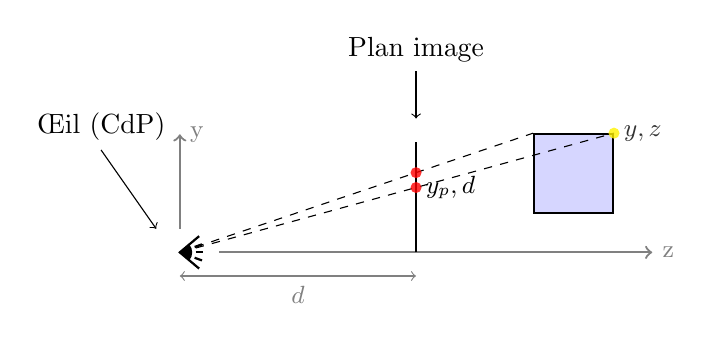
\begin{tikzpicture}
        \draw[axis,->] (0.5,0) -- (6,0) node[right] {z};
        \draw[axis,->] (0,0.3) -- (0,1.5) node[right] {y};

        \node[box,cm={1,0,0,1,(0,0)}] at (5,1) (obj) {};

        \path[draw,thick,name path=imageplan] (3,0) -- (3,1.4);

        \only<1>{
        \path[draw,thin, dashed,name path=ray1] (0,0) -- (obj.north west);
        \path [name intersections={of=imageplan and ray1,by={pt1}}];
        \fill[red,opacity=.8] (pt1) circle (2pt);
        }

        \path[draw, thin, dashed,name path=ray2] (0,0) -- (obj.north east);
        \path [name intersections={of=imageplan and ray2,by={pt2}}];
        \fill[red,opacity=.8] (pt2) circle (2pt);

        \draw[axis,thin,<->] (0,-0.3) -- (3,-0.3) node[midway,below] {$d$};

        \path[draw,thick] (40:0.32) -- (0,0) -- (-40:0.32);
        \draw[fill=black] (0,0) -- (-40:0.15) arc (-40:40:.15) -- cycle;
        \foreach \x in {-20, 0, 20} \path[draw,thick] (\x:0.2) -- (\x:0.3);

        \uncover<1>{
            \draw[<-] (-0.3,0.3) -- (-1,1.3) node[above] {\OE il (CdP)};
            \draw[<-] (3,1.7) -- (3,2.3) node[above] {Plan image};
        }

        \uncover<2->{
            \fill[yellow,opacity=.8] (obj.north east) circle (2pt) node[right,black] {\small $y,z$};
            \draw (pt2) node[right] {\small $y_p,d$};

        }
    \end{tikzpicture}

    \only<2>{
\[
    \frac{y_p}{y} = \frac{d}{z} \rightarrow y_p = \frac{d}{z}  y
\]
\[
\begin{bmatrix} y \\ z \end{bmatrix} \rightarrow \begin{bmatrix} \frac{d}{z} y \\ d \end{bmatrix} 
\]
}
    \end{center}
\end{frame}

\begin{frame}{En 3D}

    \begin{center}
    \input{sketches/projection-cube2.tex}
\only<1>{
\[
    \begin{bmatrix} 1 & 0 & 0 & 0 \\ 
                    0 & 1 & 0 & 0\\
                    0 & 0 & 1 & 0\\
                    0 & 0 & 0 & \alpha
\end{bmatrix} \begin{bmatrix} x \\ y \\ z \\ 1 \end{bmatrix}
= \begin{bmatrix} x \\ y \\ z \\ \alpha \end{bmatrix} 
\cong \begin{bmatrix} x/\alpha \\ y/\alpha \\ z/\alpha \\ 1 \end{bmatrix} 
\]
}
\only<2>{
    \[
    \begin{bmatrix} 1 & 0 & 0 & 0\\ 
                    0 & 1 & 0 & 0\\
                    0 & 0 & 1 & 0 \\
                    0 & 0 & 0 & \frac{z}{d}
\end{bmatrix} \begin{bmatrix} x \\ y \\ z \\ 1 \end{bmatrix}
= \begin{bmatrix} x \\ y \\ z \\ \frac{z}{d} \end{bmatrix} 
\cong \begin{bmatrix} \frac{dx}{z} \\ \frac{dy}{z} \\ d \\ 1 \end{bmatrix} 
\]
}

    \end{center}

\end{frame}

\begin{frame}{En 3D}
    \begin{center}
\[
    \begin{bmatrix} 1 & 0 & 0 & 0\\ 
                    0 & 1 & 0 & 0\\
                    0 & 0 & 1 & 0 \\
                    0 & 0 & 0 & \frac{z}{d}
\end{bmatrix} \begin{bmatrix} x \\ y \\ z \\ 1 \end{bmatrix}
= \begin{bmatrix} x \\ y \\ z \\ \frac{z}{d} \end{bmatrix} 
\cong \begin{bmatrix} \frac{dx}{z} \\ \frac{dy}{z} \\ d \\ 1 \end{bmatrix} 
\]

\only<1>{
\Large
Quel est le problème ?
}
\uncover<2->{
\[
    \begin{bmatrix} 1 & 0 & 0 & 0\\ 
                    0 & 1 & 0 & 0\\
                    0 & 0 & 1 & 0 \\
                    0 & 0 & \frac{1}{d} & 0
\end{bmatrix} \begin{bmatrix} x \\ y \\ z \\ 1 \end{bmatrix}
= \begin{bmatrix} x \\ y \\ z \\ \frac{z}{d} \end{bmatrix} 
\cong \begin{bmatrix} \frac{dx}{z} \\ \frac{dy}{z} \\ d \\ 1 \end{bmatrix} 
\]
}
\end{center}

\end{frame}

\begin{frame}{}
    Que représente $d$ ?
    \uncover<2>{
        La {\Medium distance focale} $f$ de notre caméra
    }
\end{frame}

%\begin{frame}{}
%
%\begin{center}
%    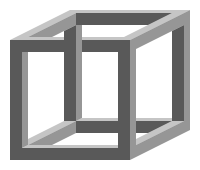
\includegraphics[width=0.8\linewidth]{impossible_cube}
%\end{center}
%
%\end{frame}

\begin{frame}{Matrice Model-View-Projection}
    \begin{center}

\only<1> {
    \input{sketches/mvp.tex}
    \[
    \mathcal{M}_{\text{MVP}}=
    \underbrace{
    \begin{bmatrix}
                    1 & 0 & 0 & 0  \\
                    0 & 1 & 0 & 0  \\
                    0 & 0 & 1 & 0  \\
                    0 & 0 & 1/f & 0
    \end{bmatrix}
    }_{\text{Matrice de projection}}
    \underbrace{
    \begin{bmatrix}
        \block(3,3){R_{cam}} & \block(1,3){T_{cam}} \\
                    &  &  &  \\
                    &  &  &  \\
                    0 & 0  & 0 & 1
    \end{bmatrix}^{-1}
    }_{\text{Matrice vue}}
    \underbrace{
    \begin{bmatrix}
        \block(3,3){R_{obj}} & \block(1,3){T_{obj}} \\
                    &  &  &  \\
                    &  &  &  \\
                    0 & 0  & 0 & 1
    \end{bmatrix}
    }_{\text{Matrice objet}}
    \]
}
\only<2>{
    \input{sketches/mvp-point.tex}
    \[
    \begin{bmatrix} x_p \\ y_p \\ f \\ 1 \end{bmatrix} \cong
    \begin{bmatrix}
                    1 & 0 & 0 & 0  \\
                    0 & 1 & 0 & 0  \\
                    0 & 0 & 1 & 0  \\
                    0 & 0 & 1/f & 0
    \end{bmatrix}
    \begin{bmatrix}
        \block(3,3){R_{cam}} & \block(1,3){T_{cam}} \\
                    &  &  &  \\
                    &  &  &  \\
                    0 & 0  & 0 & 1
    \end{bmatrix}^{-1}
    \begin{bmatrix}
        \block(3,3){R_{obj}} & \block(1,3){T_{obj}} \\
                    &  &  &  \\
                    &  &  &  \\
                    0 & 0  & 0 & 1
    \end{bmatrix}
    \begin{bmatrix} x \\ y \\ z \\ 1 \end{bmatrix}
    \]

}
    \end{center}

\end{frame}

\begin{frame}{}
    \begin{center}
    \Large
    Vous voilà équipés pour le projet.
    \end{center}
\end{frame}
%%%%%%%%%%%%%%%%%%%%%%%%%%%%%%%%%%%%%%%%%%%%%%%%%%%%%%%%%%%%%%%%%%%%%%%%%%%%%%%

\section{Rendu 3D}

\imageframe{ikea.jpg}
\imageframe{ikea1.jpg}
% this one is the (only) real photo
\imageframe{ikea3.jpg}
\imageframe{ikea2.jpg}

\begin{frame}{Rendu 3D}
    \begin{itemize}
        \item Visibilité
        \item Illumination des objets
        \item Ombres
        \item Textures
        \item Pipeline de rendu
        \item Shaders
    \end{itemize}
\end{frame}

\begin{frame}{Problème de la visibilité}
    \begin{center}
        \only<1>{
        Approche naïve: algorithme du peintre
        \includegraphics[width=0.8\linewidth]{painters_algorithm}
    }
        \only<2>{
        \includegraphics[width=0.6\linewidth]{painters_problem}
    }
    \end{center}
\end{frame}

\begin{frame}{z-buffering}
    \begin{center}
        \includegraphics[width=0.6\linewidth]{Z_buffer}
    \end{center}
\end{frame}

\begin{frame}{Illumination (1)}

    \begin{center}
        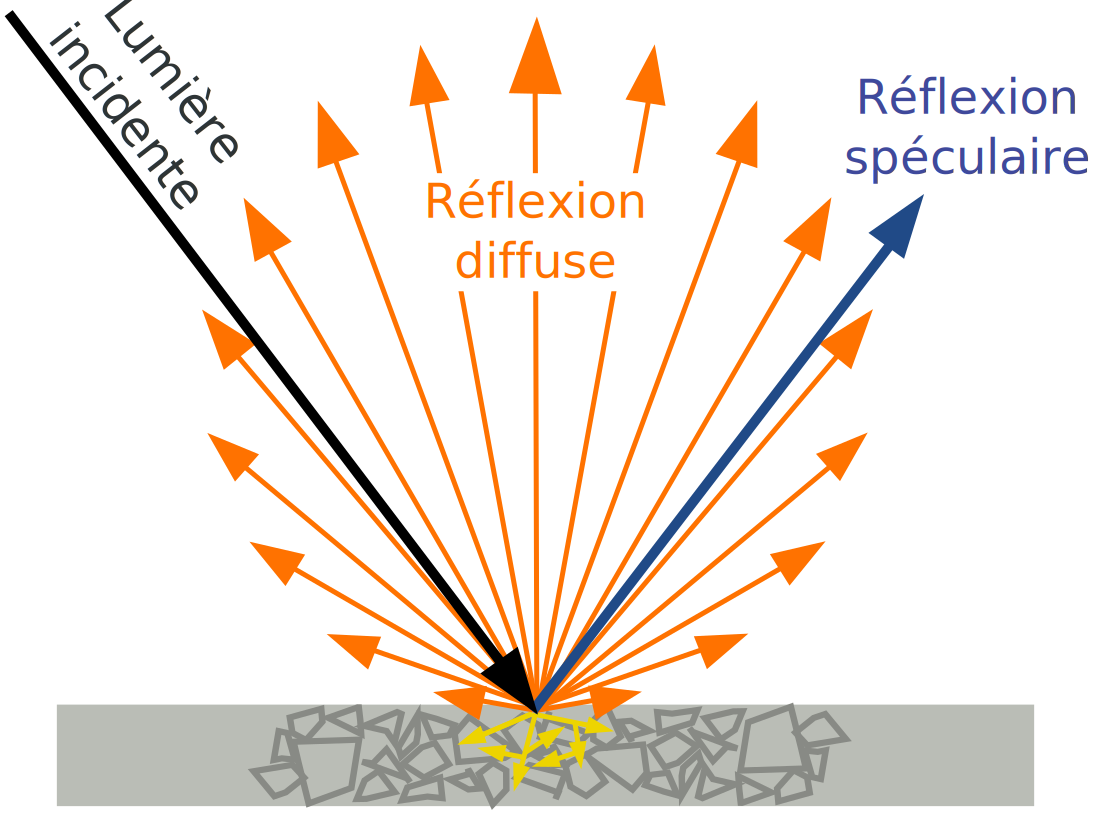
\includegraphics[width=0.8\linewidth]{diffuse_light}
    \end{center}

\end{frame}

\begin{frame}{Illumination (2)}
    Quatre sources principales d'illumination :

    \begin{itemize}
        \item {\Medium ambiante}
        \item {\Medium diffuse} (``couleur'')
        \item {\Medium spéculaire} (``reflets'')
        \item {\Medium émissive}
    \end{itemize}
    \only<1>{

    \begin{center}
        \includegraphics[width=\linewidth]{phong-model}
    \end{center}
}

    \only<2>{

    \begin{center}
        \includegraphics[width=0.6\linewidth]{3dscene}
    \end{center}
}

\end{frame}

\begin{frame}{Illumination (3)}

    \begin{center}
        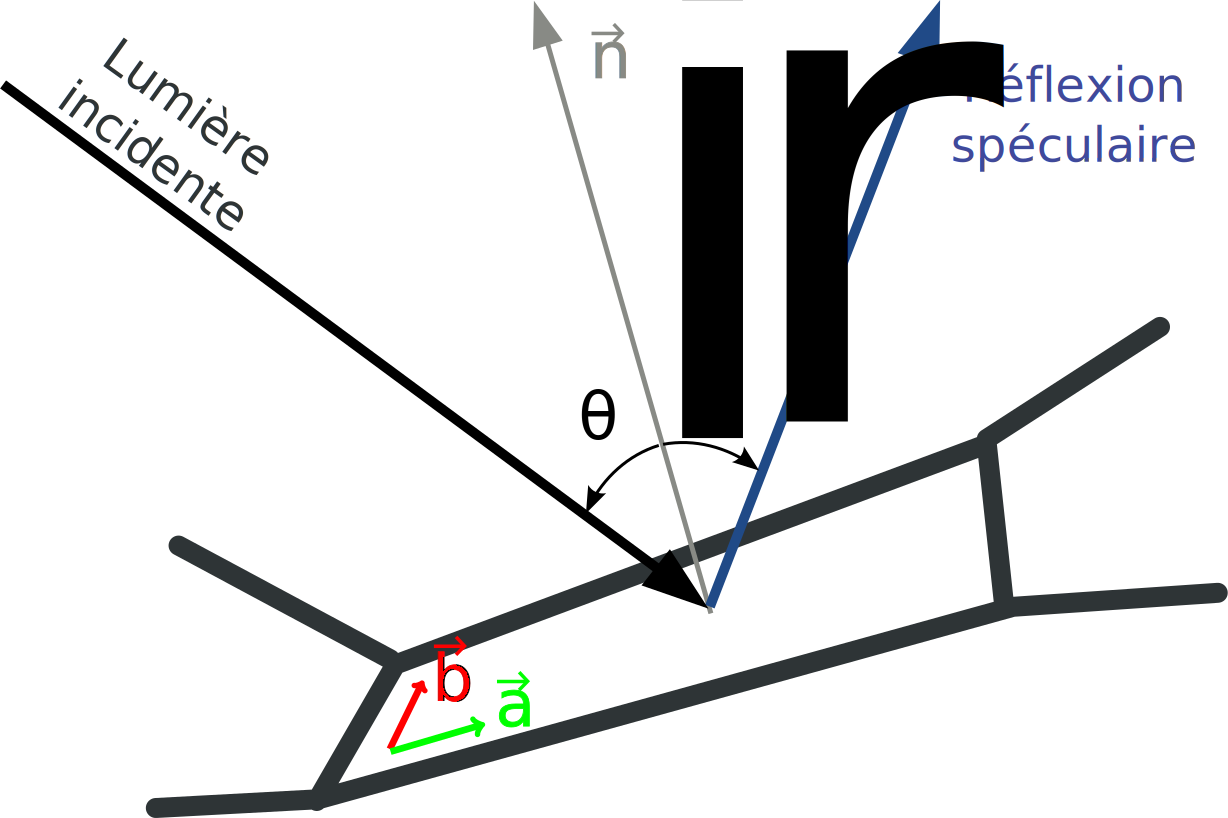
\includegraphics[width=0.6\linewidth]{specular_reflection}
    \end{center}

Si la surface est définie par deux vecteurs $\vec a$ et $\vec b$,
\[
    \vec n = \vec{a} \times \vec{b} = \colvec{3}{a_x}{a_y}{a_z} \times
    \colvec{3}{b_x}{b_y}{b_z} = \colvec{3}{a_yb_z - a_zb_y}{a_zb_x -
    a_xb_z}{a_xb_y - a_yb_x}
\]


\end{frame}

\begin{frame}{Illumination (4)}

    \begin{center}
        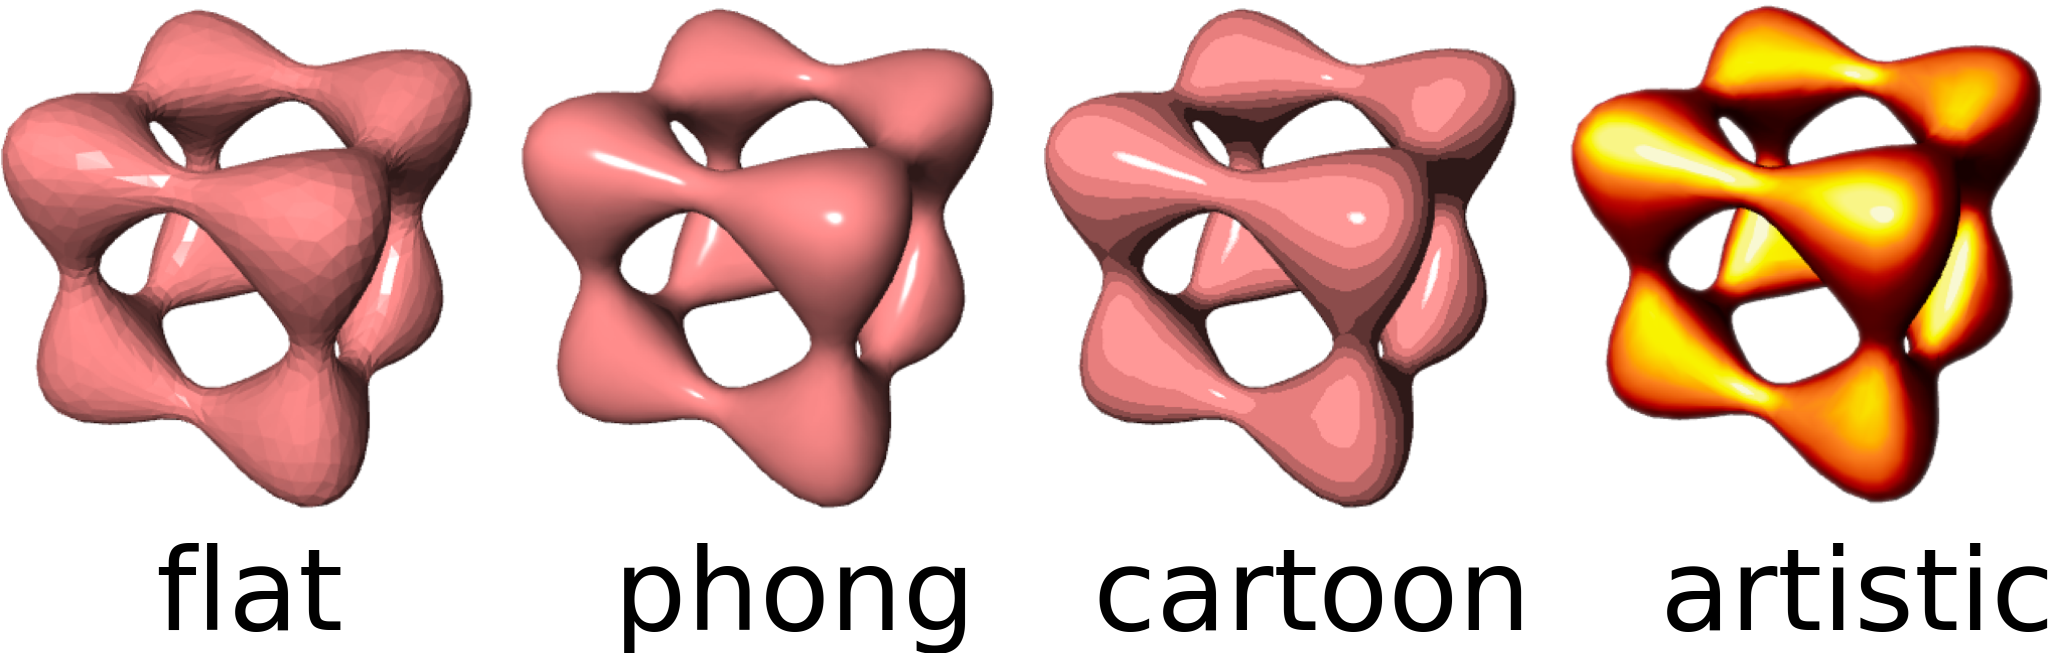
\includegraphics[width=\linewidth]{shading}
    \end{center}
\end{frame}


\begin{frame}{Ombres}
    Technique de base : {\Medium shadow mapping}\\[1em]

    {\Medium Idée clé}: voir le monde à travers la source de lumière.

    \begin{center}
        \includegraphics[width=0.8\linewidth]{shadow_mapping}
    \end{center}
\end{frame}

\imageframe{shadow-1}
\imageframe{shadow-2}
\imageframe{shadow-3}
\imageframe{shadow-4}
\imageframe{shadow-4bis}
\imageframe{shadow-5}

\begin{frame}{Textures}
    \begin{center}
        \includegraphics[width=0.3\linewidth]{sintel-opengl-transparent}
        \includegraphics[width=0.3\linewidth]{sintel-opengl-textures-transparent}
    \end{center}
\end{frame}

\imageframe{texture_diff}
\imageframe{texture_spec}
\imageframe{texture_bump}

\begin{frame}{Coordonnées de textures}
    \begin{center}

        \includegraphics[width=1\linewidth]{texture_uvmap}
    \end{center}
\end{frame}


\imageframe{cryengine3-faces}

%%%%%%%%%%%%%%%%%%%%%%%%%%%%%%%%%%%%%%%%%%%%%%%%%%%%%%%%%%%%%%%%%%%%%%%%%%%%%%%

\begin{frame}{Techniques de rendu}

    Deux grandes techniques :
    \begin{itemize}
        \item le {\Medium raytracing} (rendu de la lumière physiquement réaliste, lent)
        \item la {\Medium rasterization} (essentiellement, une projection de la géométrie)
    \end{itemize}
\end{frame}

%\begin{frame}{Raytracing}
%    Processus \emph{opposé} à celui de la projection.
%\end{frame}




{
\paper{Source: Basé sur Thorsten Thormählen, univ. Magdeburg}
\begin{frame}{Le pipeline OpenGL}

\begin{center}
\begin{tikzpicture}[
                    >=latex,
                    every edge/.style={<-, draw, very thick},
                    every node/.style={draw, font=\sf, node distance=0.5, rounded corners, align=center, inner sep=5pt,fill=hriSec3CompDark!50},
                    pic/.style={fill=none,draw=none}
                ]


    \node [fill=hriSec2Dark!50] (0,0) (vertexdata) {vertex data};
    \node [fill=hriSec2Comp!50,below =of vertexdata] (vertexshader) {per-vertex operations} edge (vertexdata);
    \node [below =of vertexshader] (primitiveassembly) {primitive assembly} edge (vertexshader);

    %\node [fill=hriSec2Dark!50,right =4 of vertexdata] (pixeldata) {pixel data};
    %\node [below =of pixeldata] (pixelops) {pixel operations} edge (pixeldata);
    %\node [below =of pixelops] (textureassembly) {texture assembly} edge (pixelops);

    \node [below =of primitiveassembly] (rasterizer) {rasterizer} edge (primitiveassembly);
    %\path[every edge] (rasterizer) -| (primitiveassembly);
    %\path[every edge] (rasterizer) -| (textureassembly);

    \node [fill=hriSec2Comp!50,below =of rasterizer] (fragshader) {per-fragment operations} edge (rasterizer);
    \node [below =of fragshader] (frame) {frame buffer} edge (fragshader);
    %\path[every edge] (frame) -| (pixelops);

    \uncover<2->{\node[pic,left=of vertexdata] {\includegraphics[width=4em]{openglpipeline_animate1.png}};}
    \uncover<3->{\node[pic,left=of vertexshader] {\includegraphics[width=4em]{openglpipeline_animate2.png}};}
    \uncover<4->{\node[pic,left=of primitiveassembly] {\includegraphics[width=4em]{openglpipeline_animate3.png}};}
    \uncover<5->{\node[pic,left=of rasterizer] {\includegraphics[width=4em]{openglpipeline_animate4.png}};}
    \uncover<6->{\node[pic,left=of fragshader] {\includegraphics[width=4em]{openglpipeline_animate5.png}};}
    \uncover<7->{\node[pic,left=of frame] {\includegraphics[width=4em]{openglpipeline_animate6.png}};}
\end{tikzpicture}
\end{center}

\end{frame}
}

\imageframe{OpenGL44PipelineMap}

\begin{frame}{Shaders}
    GPU récents: plus de 1000 cores $\Rightarrow$ parallélisation massive\\[1em]

    Pipeline programmable:
    \begin{itemize}
        \item {\Medium Vertex shader}
        \item {\Medium Fragment (ou Pixel) shader}
        \item Geometry shader
        \item Tessellation shader
    \end{itemize}

    Un {\Medium shader} est un programme écrit en GLSL (GL Shading Language,
    OpenGL) ou HLSL (High-Level Shading Language, Direct3D) et exécuté en
    parallèle sur les différents cores du GPU.
\end{frame}

\begin{frame}[fragile]{Vertex Shader pour l'illumination Phong}

\begin{glslcode}
uniform mat4 transformationMatrix;
uniform mat4 projectionMatrix;
uniform mat3 normalMatrix;
uniform vec3 light;

in vec4 position;
in vec3 normal;

out vec3 transformedNormal;
out vec3 lightDirection;
out vec3 cameraDirection;

void main() {
    vec4 transformedPosition4 = transformationMatrix*position;
    vec3 transformedPosition = transformedPosition4.xyz/transformedPosition4.w;

    transformedNormal = normalMatrix*normal;

    lightDirection = normalize(light - transformedPosition);

    cameraDirection = -transformedPosition;

    gl_Position = projectionMatrix*transformedPosition4;
}
\end{glslcode}

\end{frame}

\begin{frame}[fragile]{Fragment Shader pour l'illumination Phong}

\begin{glslcode}
uniform vec3 lightColor;
uniform float shininess;
uniform vec3 ambientColor;
uniform vec3 diffuseColor;
uniform vec3 specularColor;

in vec3 transformedNormal;
in vec3 lightDirection;
in vec3 cameraDirection;

void main() {
    color.rgb = ambientColor;

    vec3 normalizedTransformedNormal = normalize(transformedNormal);
    vec3 normalizedLightDirection = normalize(lightDirection);

    float intensity = max(0.0, dot(normalizedTransformedNormal, normalizedLightDirection));
    color.rgb += diffuseColor*lightColor*intensity;

    vec3 reflection = reflect(-normalizedLightDirection, normalizedTransformedNormal);
    float specularity = pow(max(0.0, dot(normalize(cameraDirection), reflection)), shininess);

    color.rgb += specularColor*specularity;
}
\end{glslcode}

\end{frame}



\begin{frame}{Exemple de question}

Laquelle des matrices suivantes représente la transformation 2D ``une translation
d'un vecteur $\vec t = (2,1)$ suivie d'une rotation de $\theta = 90^{\circ}$''.

\begin{itemize}
    \item $\begin{bmatrix} 0 & 1 \\ 1 & 1 \end{bmatrix}$ $\begin{bmatrix} 0 & 2 \\ 1 & 1 \end{bmatrix}$
    \item $\begin{bmatrix} 0 & 1 & -2 \\ 1 & 0 & 1 \\ 0 & 0 & 1 \end{bmatrix}$
    \item $\begin{bmatrix} 0 & 1 & -1 \\ 1 & 0 & -2 \\ 0 & 0 & 1 \end{bmatrix}$
    \item $\begin{bmatrix} 0 & 1 & -1 \\ 1 & 0 & 2 \\ 0 & 0 & 1 \end{bmatrix}$
    \item cette transformation ne peut pas être représenter sous forme
        matricielle 
\end{itemize}


\end{frame}

\begin{frame}{}
    \begin{center}
        \Large
        That's all, folk!\\[2em]
        \normalsize
        Questions : \url{severin.lemaignan@epfl.ch} \\
        Slides : \url{github.com/severin-lemaignan/intro-3d-computer-graphics}
    \end{center}
\end{frame}
\end{document}






